\subsection{A Short History of Autonomous Vehicles}

Autonomous Vehicles (a.k.a. Automated/Driverless/Unmanned/Robotic/Self-driving Vehicles) is a relatively vague concept to the public. Actually, it covers a continuum  from traditional fully human-driving automobiles to fully self-driving vehicles, as SAE classified in the Table \ref{figure:loa}.

\begin{table}[h]		
	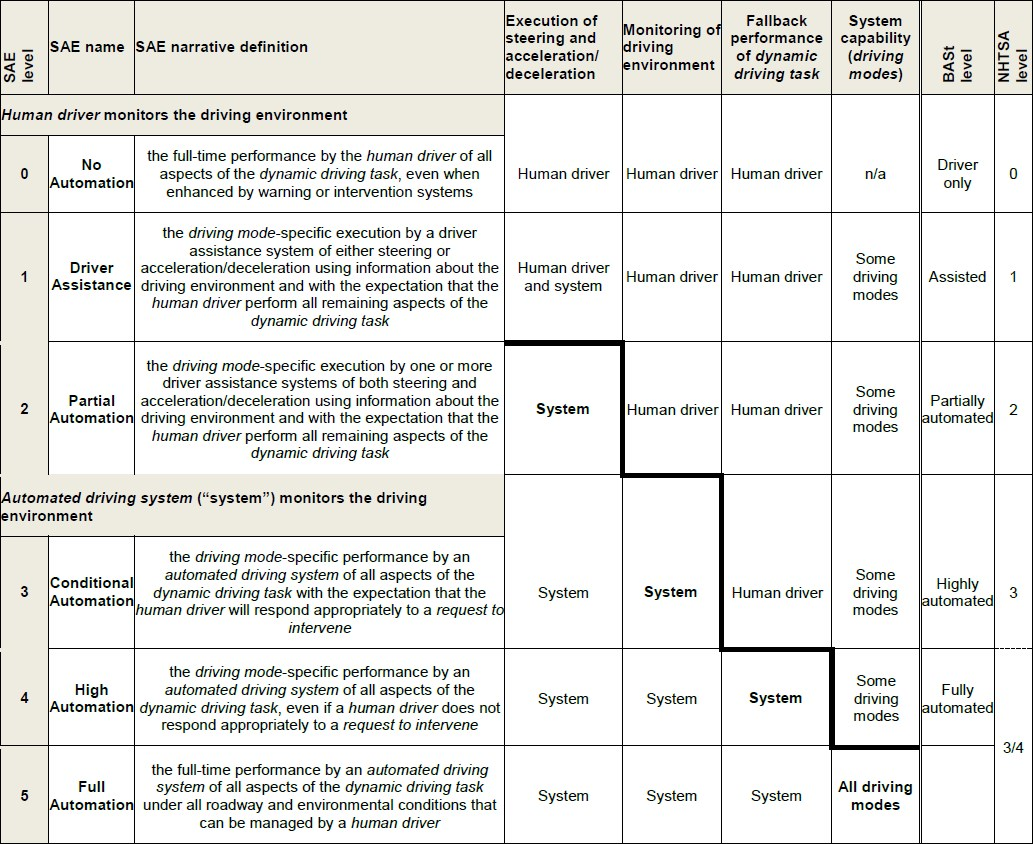
\includegraphics[width=1\textwidth]{Levels_of_Automation_2014.jpg}
	\caption{Summary of levels of driving automation\cite{J3016_201401}}
	\centering
	\label{figure:loa}
\end{table}

Contrary to the intuition, the idea of Autonomous Vehicles has a long history. The experiments of this fictional idea can be tracked back to 1920s and the technology behind it was radio control \cite{pawtc}. 

But the truly autonomous cars did not show up until 1980s, even though they could only move slowly on clear streets and required large human intervention. Mercedes-Benz demonstrated a robotic van based on saccadic vision \cite{schj}. The Autonomous Land Vehicle (ALV) project funded by The Defense Advanced Research Projects Agency (DARPA) cultivated automatic vehicles based on Computer Vision, LIDAR, and autonomous robotic control \cite{Kanade:1986:ALV:324634.325197}. Carnegie Mellon University initiatively applied neural network to control the vehicle \cite{NIPS1988_95}. 

In 1990s, huge progress was made.The VaMP from Daimler-Benz drove more than 1000 km, achieving the maximum speed of 130 km/h on a normal Pairs highway semi-autonomously \cite{schj}. The Navlab project in Carnegie Mellon University achieved a 5000 km  journey cross America with only 1.8\% human interventions \cite{nohand}. The ParkShuttle in Netherlands could autonomously navigate itself on a dedicated lane as an automated people mover \cite{parkshuttle}.In this decade, the experiments were mainly carried out in highway scenarios rather than urban scenes.

In 2000s, competitions promoted this technology a lot. One of the most famous is The DARPA Grand Challenge in U.S. who offered \$ 1 million for the first prize. In 2004, no vehicle completed the 241-km journey autonomously while 5 teams achieved this goal in 2005 \cite{Buehler2007}. And in Grand Challenge III 2007 , known as Urban Challenge, 6 vehicles  finished the event which was a 96 km urban route involving with traffic regulations and other vehicles \cite{Buehler2009}.

In 2010s,  Autonomous Driving Technology starts to take off. Numerous events and projects have been carried out and considerable companies, universities, and research centres have engaged into this field. Based on the progress made before, many autonomous vehicle systems are being tested or even brought into production.  Notable events covers the VisLab Intercontinental Autonomous Challenge in 2010 \cite{doi:10.1504/IJVAS.2012.051250} and the Intelligent Vehicle Future  Challenges from 2009 to 2013 \cite{newlet00}. In industry, Tesla Motor released AutoPilot  that is able to perform automated parking and lane control with autonomous driving, braking and speed adjustment in 2014, and  Audi started the first production car, A8,  reaching Level 3 of Automation in 2017 \cite{historyad}.

Based of the efforts in the last decades, Autonomous Driving  gradually transform from dream to reality. Its bonus covers safety guarantee, congestion reduction, land use efficiency, energy and emission reduction, economic benefits and so on. However, the Level 5 vehicles are so far from maturity that the research and development are in high demand.
